\section{Introduction}

  \par Bike shares are riding a wave of popularity in the intermodal transit planning community. Through bike sharing systems in a city, people are able to rent a bike from a one location and return it to a different place on an as-needed basis. The number of bike share systems, defined as publicly-available systems with at least 10 stations and 100 bikes, has steadily increased year-over-year, from four systems in 2010 to 55 systems in 2016 across U.S, with over 42,000 bikes available in cities of all sizes. In addition, 80\% of systems that have been in operation for more than a year have expanded since they launched. 2016 saw the launch of two large systems in major cities: BIKETOWN in Portland, OR and Metro Bike Share\cite{bike} in Los Angeles, CA. The number of bikes in the nation also increased substantially, up 30\%, as existing large systems have continued to grow.
  \par The growth of bike share shows no signs of stopping. A number of U.S. cities, such as Detroit, New Haven, and New Orleans, have either selected vendors or are planning to launch systems, and many existing systems are also rolling out major expansions. : New York's City Bike is adding another 2,000 bikes, for a total of 12,000; Houston is more than tripling in size to over 100 stations; and the San Francisco Bay Area is expanding from a 700 to a 7,000 bike system. Here in our assignment, we conduct a case study based on the bike sharing data on the Metro Bike Share System in Los Angeles. We try to forecast the bike sharing demand to help design and expand the bike sharing system in LA. 




  \par In our analysis, what did we learned from? // We reviewed... discussed...

  \par Our three/four/five models and brief description. [name and principles.] We evaluate based on RMSE..... We also discuss...


\section{Data}
  \par Describe the dataset.

  ??? The data generated by these systems makes them attractive for researchers because the duration of travel, departure location, arrival location, and time elapsed is explicitly recorded. Bike sharing systems therefore function as a sensor network, which can be used for studying mobility in a city. In this competition, participants are asked to combine historical usage patterns with weather data in order to forecast bike rental demand in the Capital Bikeshare program in Washington, D.C.

\section{Predictive Task}

\section{Models and Methodology}

\section{Literature}

\section{Results and Conclusions}

% The \textit{proceedings} are the records of a conference.\footnote{This
  % is a footnote}
% \subsection{Type Changes and {\itshape Special} Characters}

% \subsection{Math Equations}

% \subsubsection{Inline (In-text) Equations}

% \begin{table}
%   \caption{Frequency of Special Characters}
%   \label{tab:freq}
%   \begin{tabular}{ccl}
%     \toprule
%     Non-English or Math&Frequency&Comments\\
%     \midrule
%     \O & 1 in 1,000& For Swedish names\\
%     $\pi$ & 1 in 5& Common in math\\
%     \$ & 4 in 5 & Used in business\\
%     $\Psi^2_1$ & 1 in 40,000& Unexplained usage\\
%   \bottomrule
% \end{tabular}
% \end{table}



% \begin{table*}
%   \caption{Some Typical Commands}
%   \label{tab:commands}
%   \begin{tabular}{ccl}
%     \toprule
%     Command &A Number & Comments\\
%     \midrule
%     \texttt{{\char'134}author} & 100& Author \\
%     \texttt{{\char'134}table}& 300 & For tables\\
%     \texttt{{\char'134}table*}& 400& For wider tables\\
%     \bottomrule
%   \end{tabular}
% \end{table*}
% % end the environment with {table*}, NOTE not {table}!

% It is strongly recommended to use the package 
% and follow its main principles of typography with respect to tables:
% \begin{enumerate}
% \item Never, ever use vertical rules.
% \item Never use double rules.
% \end{enumerate}
% It is also a good dingsidea not to overuse horizontal 


% \subsection{Figures}


% \begin{figure}
% 
\includegraphics{fly}
% \caption{A sample black and white graphic.}
% \end{figure}

% \begin{figure}
% 
\includegraphics[height=1in, width=1in]{fly}
% \caption{A sample black and white graphic
% that has been resized with the \texttt{includegraphics} command.}
% \end{figure}



% \begin{figure*}
% 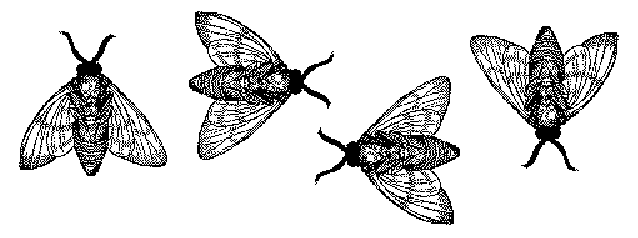
\includegraphics{flies}
% \caption{A sample black and white graphic
% that needs to span two columns of text.}
% \end{figure*}


% \begin{figure}
% 
\includegraphics[height=1in, width=1in]{rosette}
% \caption{A sample black and white graphic that has
% been resized with the \texttt{includegraphics} command.}
% \end{figure}


% \end{document}  % This is where a 'short' article might terminate

